\chapter{Introduction}

In the last decade, neuroscience has benefited from simulating nerve cell behaviour or neural networks. The simulation made use of large-scale and high-precision experimental methods of data acquisition to develop fact-based tools that helped understand brain functions and diseases \cite{MARKRAM201139}. Due to the amount of data collected, the simulations are done with supercomputers integrating different levels of simulation.
\begin{wrapfigure}{r}{0.25\textwidth}
    \centering
    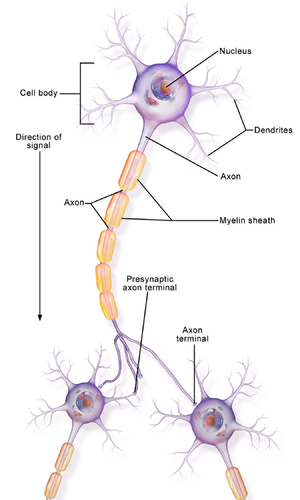
\includegraphics[width=0.25\textwidth]{setup/img/NeuronParts.png}
    \caption{A sketch of how a neuron may look like \cite{wiki:interneurons}}
    \label{fig:NeuronParts}
\end{wrapfigure}

A human brain consists of 100 billion neurons \cite{HERCULANO2012} of different types depending on their function, shape and other factors. In physiology, a neuron consists of a cell body with the nucleus, dendrites and axon, as seen in the figure \ref{fig:NeuronParts}. From a morphological perspective, a neuron is a tree. The neuron is divided into compartments. Every compartment has only one parent and can have several children (typically no more than 2). The tree's root represents the soma, which can be represented by one compartment or several. 

A point where the distance between two neurons is lower than a certain threshold defines a touchpoint. If there is a touchpoint, then a synapse can emerge. A synapse is a structure that permits a neuron to pass an electrical or chemical signal to another neuron. There are different types of synapses. The most common is axodendritic. But there are also other types, depending on which parts of the neurons are in touch, such as axo-axonic, dendro-dendritic, axo-secretory, somatodendritic, dendro-somatic, and somato-somatic synapses.

One usual workflow consists of first doing a single-cell morphology reconstruction, then building a local network finding touchpoints and selecting possible synapses \cite{Reimann2015-ys} and finally simulating the signals exchange. Usually, a neuron has 1000 inputs that fire at an average rate of 10 Hz and each connection requires around ten instructions \cite{Furber2006}. These make the simulation in real-time of a human brain infeasible even with terascale computers.

When building a local network, space-partitioning structures are used for faster searches of touchpoints. This thesis will consider Kd-trees as the space-partitioning structure as previous research showed it performs better for this task \cite{Adamsson_Vorkapic_2016}. A Kd-tree is a space-partitioning data structure for organizing points in a k-dimensional space by dividing the Euclidian space into two convex sets using hyperplanes. The methods that divides the space in two subsets are called binary space partitioning (BSP). Other examples of BSP are Octrees and Quadtrees. Some applications of BSP are robotics, computer graphics, and computer-aided design.

The field of computer graphics uses a technique for rendering a scene called ray-tracing. This technique models light transport along the stage to get the image. Although ray-tracing generates realistic images, it has a high computational cost. Computer scientists developed several techniques to reduce the high computational cost, for instance, BSP \cite{Fuchs1980}. Also, they introduced the usage of kd-trees and heuristics to improve the performance\cite{WaldHavran06, Yucheng, LinjiaSaeidMajid, Bentley, 7169256}.

\section{Problem statement}
This project aims to compare different heuristics used in computer graphics concerning performance. We will measure the performance of the heuristics in terms of execution time for building the kd-trees and for querying and random access memory (RAM) usage. These measurements will occur during typical scenarios of data-driven reconstruction of a neural network. Therefore, this thesis aims to investigate the following:

\textbf{How does the usage of heuristics in Kd-trees affect the performance of touch dectetion in neuronal morphometrics? }

\section{Scope and delimitations}
This thesis will focus on

\section{Thesis outline}
The background (Chapter \ref{chapter:background}) presents the used data structure and relevant algorithms as well as the libraries used in this thesis. The methods (Chapter \ref{chapter:methods}) explain in detail how measurements were made and the motivations for choices made. The measurements are then presented in the result chapter (Chapter \ref{chapter:results}) with the corresponding analysis. Subsequently, the results are discussed in the discussion chapter (Chapter \ref{chapter:discussion}) and a conclusion is presented  (Chapter \ref{chapter:conclusion}).
